\section{Background of the Study}



\section{Prior Studies}
\begin{table}[ht]
	\begin{center}
		\caption{Different Battery Types of Quadrotors/UAV}
	\begin{tabular}{|c|c|}
		\hline
		Type of Quadrotor/UAV                                                                   & Battery Type                                                                                             \\ \hline
		\begin{tabular}[c]{@{}c@{}}Small-size Rotary-Wing\\ Electrical UAV\end{tabular}         & Uses Lithium Polymer Batteries                                                                           \\ \hline
		\begin{tabular}[c]{@{}c@{}}Wireless Battery Charging\\ System for Drones\end{tabular}   & \begin{tabular}[c]{@{}c@{}}Uses wireless power transmission\\ via capacitive power transfer\end{tabular} \\ \hline
		\begin{tabular}[c]{@{}c@{}}Fuzzy energy management\\ for UAVs\end{tabular}              & \begin{tabular}[c]{@{}c@{}}Uses supercapacitors for power \\ optimization technique\end{tabular}         \\ \hline
		Flying by the Sun only                                                                  & Uses Solar Panel only                                                                                    \\ \hline
		\begin{tabular}[c]{@{}c@{}}Energy Efficient Sun \\ Synchronous Solar Panel\end{tabular} & \begin{tabular}[c]{@{}c@{}}Uses solar panel which moves\\ according to sunlight direction\end{tabular}   \\ \hline
	\end{tabular}
\end{center}
\end{table}
\section{Problem Statement}

\section{Objectives}

\subsection{General Objective(s)}


\subsection{Specific Objectives}
\begin{enumerate}
\item 

\item 

\item 

\end{enumerate}



\section{Significance of the Study}




\section{Assumptions, Scope and Delimitations}



\section{Description and Methodology \documentType}



\begin{figure}[ht]
	\centering
	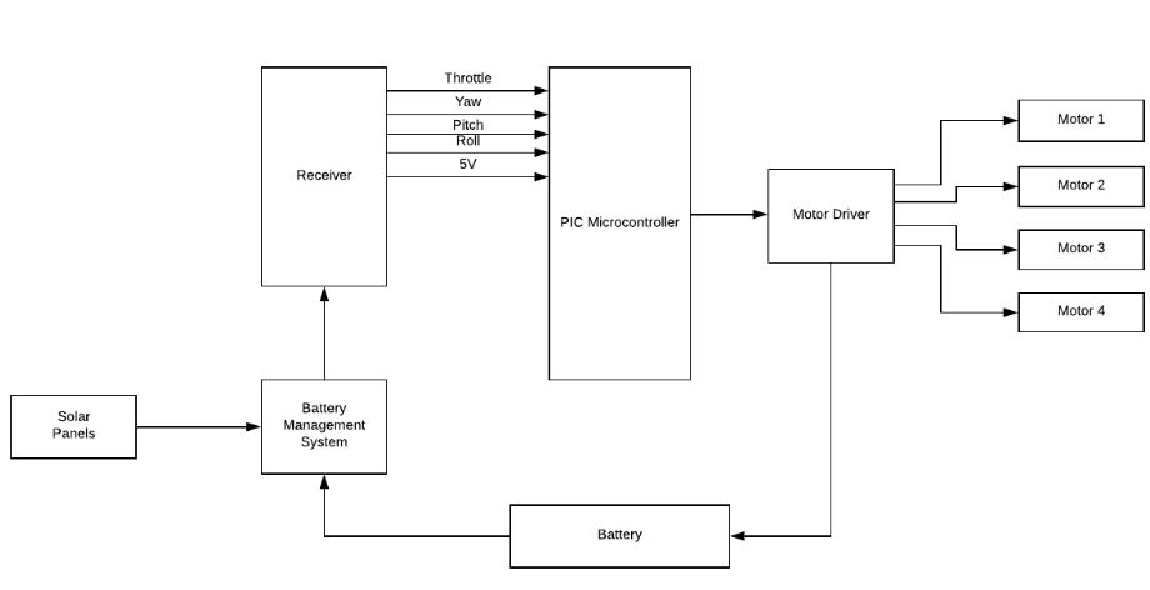
\includegraphics[height=35ex]{blockdiag}
	\caption{Block Diagram of Quadrotor}
\end{figure}




\begin{figure}[ht]
	\centering
	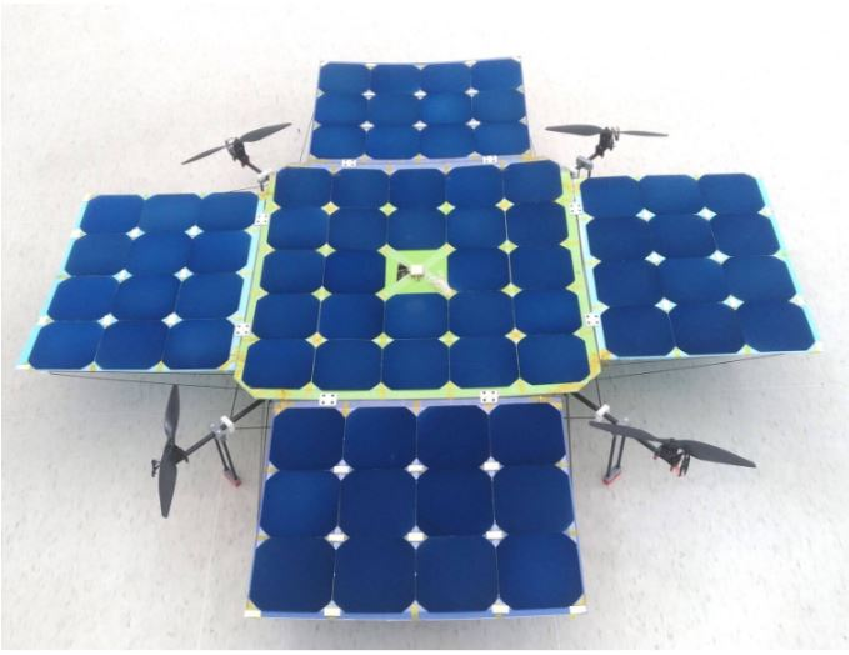
\includegraphics[height=35ex]{frame}
	\caption{Proposed Frame of Quadrotor}
\end{figure}
This is how the researchers will do the construction of the quadrotor in Fig. 1.1 and the frame wil be designed like in Fig. 1.2
\ifFinished
\else
\newpage
\section{Overview of the Thesis}
\subsection{Individual Gantt Chart}
\begin{figure}[ht]
	\centering
	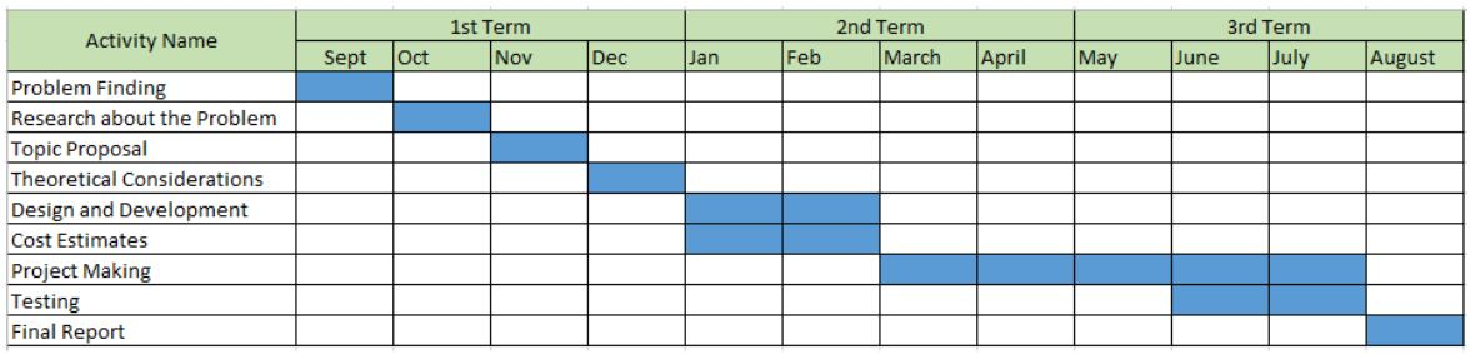
\includegraphics[height=18ex]{gantt1}
	\caption{Gantt Chart 1}
\end{figure}

\begin{figure}[ht]
	\centering
	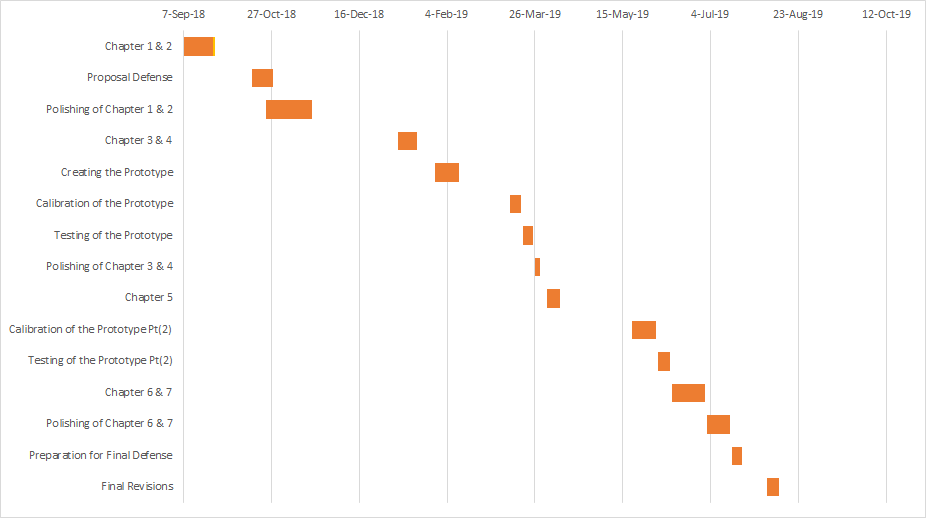
\includegraphics[height=28ex]{gantt2}
	\caption{Gantt Chart 2}
\end{figure}

\begin{figure}[ht]
	\centering
	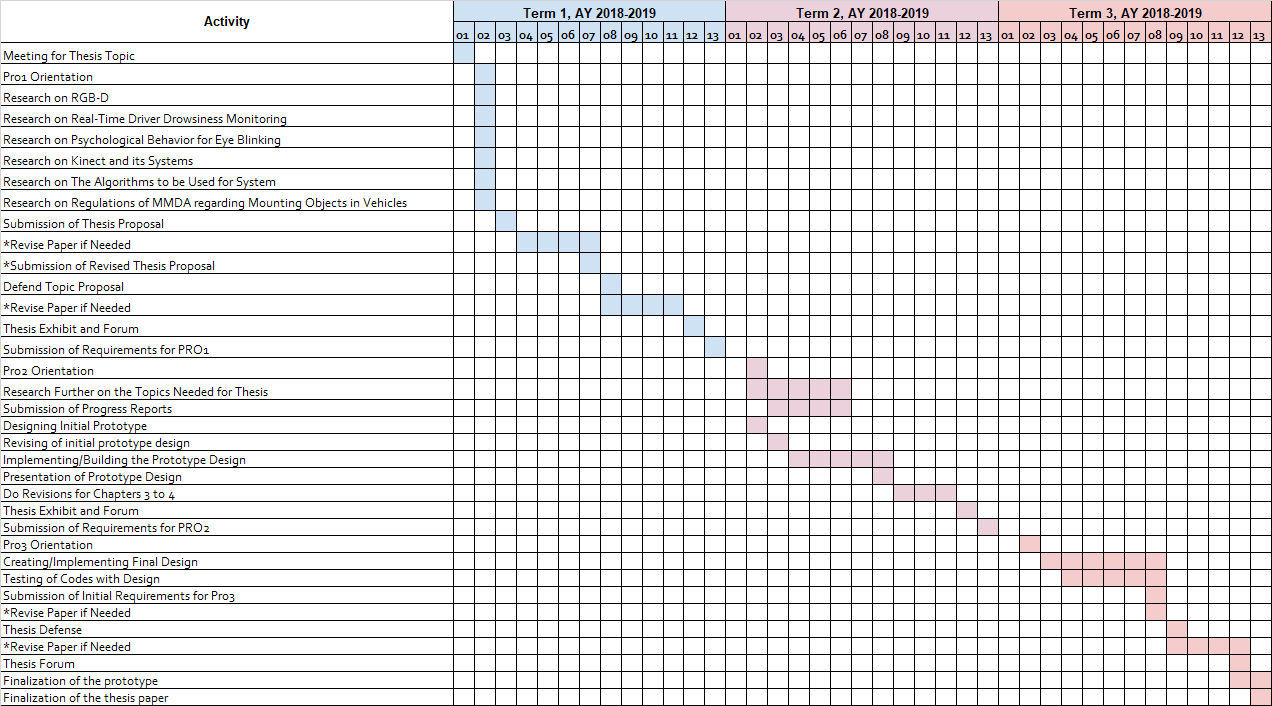
\includegraphics[height=45ex]{gantt3}
	\caption{Gantt Chart 3}
\end{figure}

\begin{figure}[ht]
	\centering
	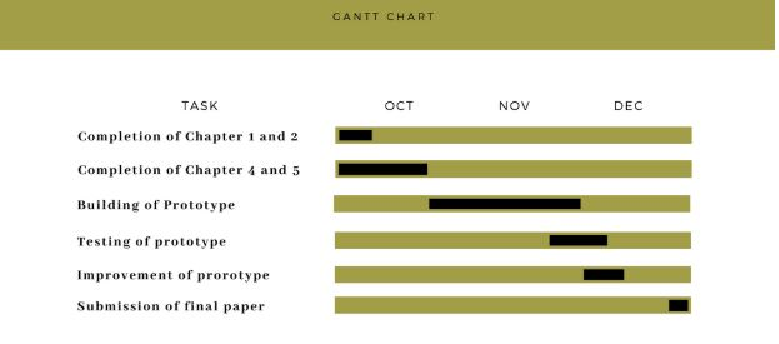
\includegraphics[height=35ex]{gantt4}
	\caption{Gantt Chart 4}
\end{figure}
\ifPhD
\section{Publication Plan}
\graytx{\blindtext}
\fi

\fi



